% Wcash Protocol Specification
% Modeled on the layout and conventions of the Zcash Protocol Specification.
% Build with XeLaTeX or pdfLaTeX (run twice).
\documentclass[10pt,letterpaper]{article}
\usepackage[letterpaper,top=0.9in,bottom=0.9in,left=0.95in,right=0.95in,footskip=0.4in]{geometry}
\usepackage{iftex}
\usepackage{amsmath,amsthm,mathtools}
\ifPDFTeX
  \IfFileExists{lmodern.sty}{\usepackage[T1]{fontenc}\usepackage{lmodern}}{}
  \usepackage{amssymb}
\else
  \usepackage{fontspec}
  \usepackage{unicode-math}
  \setmathfont{Latin Modern Math}
\fi
\usepackage[protrusion=true,expansion=false]{microtype}
\usepackage{tikz}
\usetikzlibrary{arrows.meta,positioning,calc}
\usepackage{array,tabularx,longtable}
\usepackage{enumitem}
\usepackage{caption}
\usepackage{float}
\usepackage[hidelinks,bookmarksnumbered=true,pdftitle={Wcash Protocol Specification}]{hyperref}

\setlength{\parindent}{0pt}
\setlength{\parskip}{0.55em plus 0.15em}
\emergencystretch=2em
\pagestyle{plain}
\setlist{itemsep=0.15em,topsep=0.2em,parsep=0pt}
\setlist[itemize]{leftmargin=1.6em}
\setlist[enumerate]{leftmargin=2em}
\captionsetup{font=small,labelfont=bf,labelsep=period}
\setcounter{tocdepth}{2}
\renewcommand\arraystretch{1.15}

% ---------------------------------------------------------------- conventions
\newcommand\term[1]{\textsl{#1}}
\newcommand\MUST{\textsc{must}}
\newcommand\MUSTNOT{\textsc{must not}}
\newcommand\SHOULD{\textsc{should}}
\newcommand\SHOULDNOT{\textsc{should not}}
\newcommand\MAY{\textsc{may}}
\newcommand\RECOMMENDED{\textsc{recommended}}
\newcommand\typ{\mathrel{\vcentcolon}}
\newcommand\B{\mathbb{B}}
\newcommand\BY{\mathbb{B}\kern-0.1em\mathbb{Y}}
\newcommand\Nat{\mathbb{N}}
\newcommand\fn[1]{\mathsf{#1}}
\newcommand\cat{\mathbin{\|}}
\newcommand\ascii[1]{\text{\textquotedblleft\texttt{#1}\textquotedblright}}
\newcommand\secref[1]{\S\,\ref{#1} `\nameref{#1}' on page~\pageref{#1}}
\newcommand\rules[1]{\par\textbf{#1}}
\newcolumntype{Y}{>{\raggedright\arraybackslash}X}
\newcolumntype{L}[1]{>{\raggedright\arraybackslash}p{#1}}

\theoremstyle{plain}
\newtheorem{theorem}{Theorem}[subsection]

\tikzset{>={Stealth[length=4pt,width=3.4pt]}}

\begin{document}

% =====================================================================
%  TITLE AND ABSTRACT
% =====================================================================
\begin{center}
{\LARGE\bfseries Wcash Protocol Specification\par}
\vspace{0.6em}
{\large Version 2026.1.0 [Mainnet]\par}
\vspace{0.8em}
w.cash\par
\vspace{0.4em}
September 18, 2026\par
\end{center}
\vspace{0.6em}

\textbf{Abstract.} Wcash is a cryptocurrency derived from the Zcash protocol. It shares Zcash's transaction format, its shielded payment protocol, and its Equihash proof of work, and it runs as an independent block chain secured by auxiliary proof of work reused from Zcash. A Zcash block header whose coinbase commits to a Wcash block, and whose hash meets the Wcash target, proves work for that Wcash block. This specification defines the Wcash consensus protocol, including block identity, the auxiliary proof-of-work format and its validation, difficulty adjustment, the block subsidy, coinbase rules, and the genesis block. Protocol differences from Zcash are also explained.

\textbf{Keywords:} auxiliary proof of work, cryptocurrency, emission schedule, financial privacy, merged mining, proof of work.

\tableofcontents
\clearpage

% =====================================================================
\section{Introduction}\label{sec:intro}
% =====================================================================

Wcash is a cryptocurrency derived from the Zcash protocol [Zcash-Protocol], which is itself an implementation of the Decentralized Anonymous Payment scheme Zerocash [BCGGMTV2014]. Wcash keeps Zcash's transparent payment scheme, its Ironwood shielded payment protocol, and its version 6 transaction format. It replaces the parts of Zcash that define an independent network: block identity, the genesis block, network identifiers, address encodings, consensus branch identifiers, the proof-of-work check, difficulty adjustment, and the block subsidy.

A Wcash block carries no Equihash solution of its own. It carries an \term{auxiliary proof of work}: a Zcash block header with a valid Equihash solution, together with Merkle paths showing that the header commits to the Wcash block. Any Zcash miner can therefore secure Wcash with the same work it performs for Zcash, and one solution can produce a valid block on both chains.

In this document, technical terms for concepts that play an important role in Wcash are written in slanted text. Italics are used for emphasis. The symbol \S{} precedes section numbers in cross-references.

The key words \MUST, \MUSTNOT, \SHOULD, \SHOULDNOT, \RECOMMENDED, and \MAY{} in this document are to be interpreted as described in [RFC-2119] when they appear in small capitals. They may also appear in lower case as plain English words, without their normative meaning.

Where this document is silent, the rules of [Zcash-Protocol] for the NU6.3 network upgrade apply, as modified by \secref{sec:consensus}. Rules inherited without change are generally not restated.

This specification is structured as follows:
\begin{itemize}
\item Notation: definitions of notation used throughout the document;
\item Concepts: the principal abstractions needed to understand the protocol;
\item Abstract Protocol: the merged-mining scheme and its security requirements;
\item Concrete Protocol: how the functions and encodings of the abstract protocol are instantiated;
\item Network Upgrades: the upgrades active on Wcash networks;
\item Consensus Changes from Zcash: how Wcash differs from Zcash at the consensus layer;
\item Merged Mining Considerations: non-normative guidance for pools, and an analysis of double spending.
\end{itemize}

\subsection{Caution}\label{sec:caution}

Wcash security depends on consensus. A program that diverges from consensus weakens or loses the security of every user who relies on it, and the cause of the divergence does not matter: it could be a bug, an error in this document, or other software on the network behaving unexpectedly.

A specification of intended behaviour is nevertheless essential for security analysis, for understanding the protocol, and for independent implementations. Errors in this specification should be reported to the Wcash project through \url{https://w.cash}.

\subsection{High-level Overview}\label{sec:overview}

The following overview gives a concise summary of the ideas behind the protocol for readers familiar with Zcash. It is not part of the normative specification.

All value in Wcash belongs to a \term{chain value pool}: the \term{transparent pool} or the \term{Ironwood pool}. Transparent value works as in Bitcoin and Zcash, with public addresses and amounts. Value in the Ironwood pool is carried by \term{notes}, whose commitments and nullifiers are revealed on the block chain while their values and recipients stay hidden, exactly as specified for Zcash. The older Zcash pools are not used.

Wcash blocks are found by \term{merged mining}. A mining pool builds a Zcash block whose coinbase ends with a 44-byte \term{carrier} committing to a Wcash \term{candidate block}. Each Equihash solution for that Zcash header is compared with two targets. If the header hash meets the Wcash target, the pool attaches an auxiliary proof of work to the candidate and broadcasts a Wcash block. If it meets the Zcash target, the pool broadcasts the Zcash block as usual. Because Zcash transaction identifiers exclude input scripts [ZIP-244], the proof links the coinbase to the parent header twice, once through the transaction tree and once through the authorizing-data tree (Figure~\ref{fig:paths}).

Each Wcash block pays its miner the whole block subsidy plus fees. The subsidy follows a time-scaled version of Monero's smooth emission curve [vanSaberh2013], preceded by a slow start and followed by a permanent tail.

\begin{figure}[H]
\centering
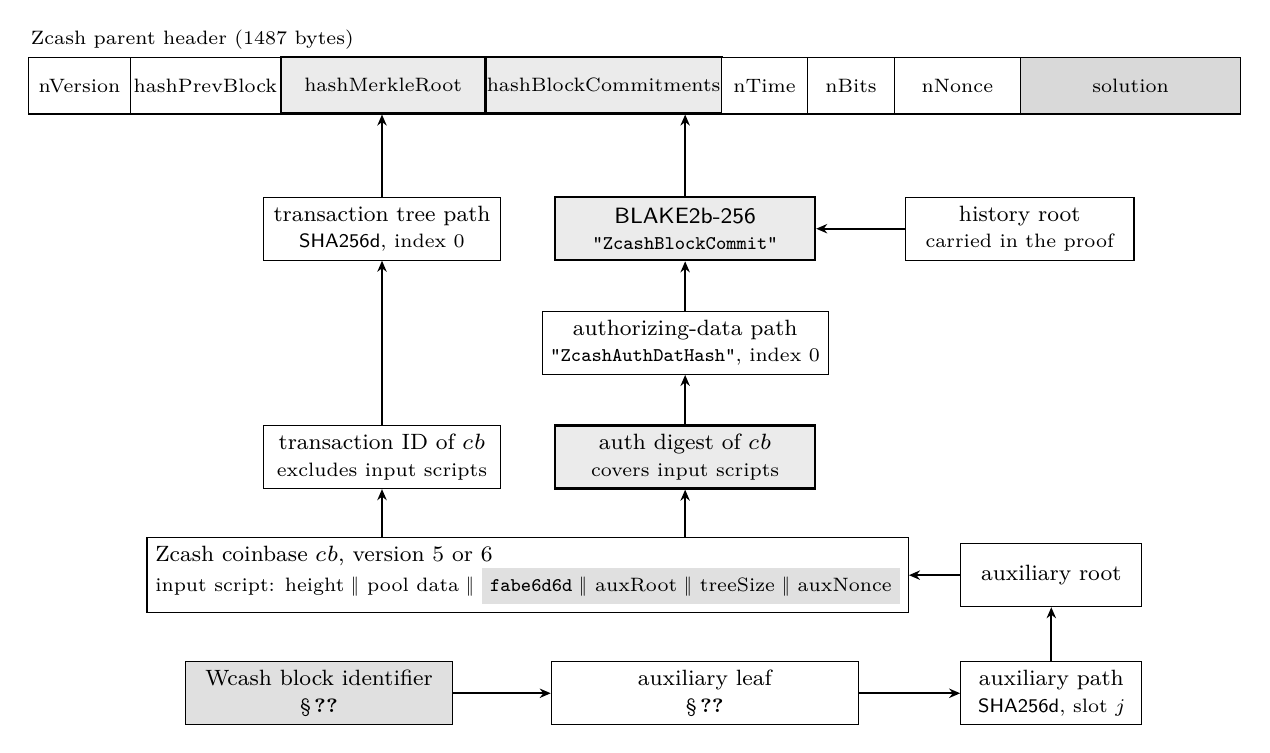
\begin{tikzpicture}[
   fld/.style={draw,minimum height=0.72cm,anchor=south west,inner sep=0,font=\scriptsize,align=center,fill=white},
   pb/.style={draw,align=center,inner sep=3pt,minimum height=0.8cm,font=\footnotesize,fill=white},
   hot/.style={fill=black!8,line width=0.8pt},
   up/.style={-{Stealth[length=4pt,width=3.4pt]},line width=0.6pt},
   lbl/.style={font=\scriptsize,inner sep=1pt}]
  \node[anchor=south west,lbl] at (0,6.78) {Zcash parent header (1487 bytes)};
  \node[fld,minimum width=1.3cm] at (0,6.0) {nVersion};
  \node[fld,minimum width=1.9cm] at (1.3,6.0) {hashPrevBlock};
  \node[fld,minimum width=2.6cm,fill=black!8,line width=0.8pt] (hm) at (3.2,6.0) {hashMerkleRoot};
  \node[fld,minimum width=3.0cm,fill=black!8,line width=0.8pt] (hc) at (5.8,6.0) {hashBlockCommitments};
  \node[fld,minimum width=1.1cm] at (8.8,6.0) {nTime};
  \node[fld,minimum width=1.1cm] at (9.9,6.0) {nBits};
  \node[fld,minimum width=1.6cm] at (11.0,6.0) {nNonce};
  \node[fld,minimum width=2.8cm,fill=black!15] at (12.6,6.0) {solution};
  \node[pb,minimum width=3.0cm] (tb) at (4.5,4.55) {transaction tree path\\{\scriptsize $\fn{SHA256d}$, index 0}};
  \node[pb,minimum width=3.0cm] (tx) at (4.5,1.65) {transaction ID of $cb$\\{\scriptsize excludes input scripts}};
  \node[pb,hot,minimum width=3.3cm] (bc) at (8.35,4.55) {$\fn{BLAKE2b\text{-}256}$\\{\scriptsize \texttt{"ZcashBlockCommit"}}};
  \node[pb,minimum width=2.9cm] (hr) at (12.6,4.55) {history root\\{\scriptsize carried in the proof}};
  \node[pb,minimum width=3.3cm] (ab) at (8.35,3.1) {authorizing-data path\\{\scriptsize \texttt{"ZcashAuthDatHash"}, index 0}};
  \node[pb,hot,minimum width=3.3cm] (ad) at (8.35,1.65) {auth digest of $cb$\\{\scriptsize covers input scripts}};
  \node[pb,minimum width=8.2cm,align=left] (cb) at (6.35,0.15) {Zcash coinbase $cb$, version 5 or 6\\{\scriptsize input script: height $\cat$ pool data $\cat$ \colorbox{black!12}{\texttt{fabe6d6d} $\cat$ auxRoot $\cat$ treeSize $\cat$ auxNonce}}};
  \node[pb,minimum width=2.3cm] (ar) at (13.0,0.15) {auxiliary root};
  \node[pb,minimum width=2.3cm] (abr) at (13.0,-1.35) {auxiliary path\\{\scriptsize $\fn{SHA256d}$, slot $j$}};
  \node[pb,minimum width=3.9cm] (lf) at (8.6,-1.35) {auxiliary leaf\\{\scriptsize \S\,\ref{sec:auxtree}}};
  \node[pb,fill=black!12,minimum width=3.4cm] (id) at (3.7,-1.35) {Wcash block identifier\\{\scriptsize \S\,\ref{sec:blockid}}};
  \draw[up] (tb.north) -- (tb.north |- hm.south);
  \draw[up] (tx.north) -- (tb.south);
  \draw[up] (bc.north) -- (bc.north |- hc.south);
  \draw[up] (hr.west) -- (bc.east);
  \draw[up] (ab.north) -- (bc.south);
  \draw[up] (ad.north) -- (ab.south);
  \draw[up] (cb.north -| tx.south) -- (tx.south);
  \draw[up] (cb.north -| ad.south) -- (ad.south);
  \draw[up] (ar.west) -- (cb.east);
  \draw[up] (abr.north) -- (ar.south);
  \draw[up] (lf.east) -- (abr.west);
  \draw[up] (id.east) -- (lf.west);
\end{tikzpicture}
\caption{Authentication paths of an auxiliary proof of work. Arrows point from committed data toward the commitment that contains it.}
\label{fig:paths}
\end{figure}

% =====================================================================
\section{Notation}\label{sec:notation}
% =====================================================================

$\B$ means the type of bit values, i.e.\ $\{0, 1\}$. $\BY$ means the type of byte values, i.e.\ $\{0\,..\,255\}$.

$\Nat$ means the type of nonnegative integers. $\Nat^+$ means the type of positive integers.

$x \typ T$ is used to specify that $x$ has type $T$. A cartesian product type is denoted by $S \times T$, and a function type by $S \to T$.

$T^{[\ell]}$, where $T$ is a type and $\ell$ is an integer, means the type of sequences of length $\ell$ with elements in $T$. $\BY^{[\Nat]}$ means the type of byte sequences of arbitrary length.

$\fn{length}(S)$ means the number of elements in $S$.

$\mathtt{0x}$ followed by a string of hexadecimal digits means the corresponding integer. $[\mathtt{0x00}]^{\ell}$ means the sequence of $\ell$ zero bytes.

$\ascii{...}$ means the given string represented as a sequence of bytes in US-ASCII.

$a \cat b$ means the concatenation of sequences $a$ then $b$.

$\fn{le32}(x)$, for $x \typ \{0\,..\,2^{32}-1\}$, means the 4-byte little-endian encoding of $x$.

$\fn{rev}(S)$, for $S \typ \BY^{[32]}$, means the sequence $S$ with its bytes in reverse order.

$\lfloor x \rfloor$ means the largest integer $\le x$. $a \bmod q$ means the remainder on dividing $a$ by $q$.

$\{a\,..\,b\}$ means the set of integers from $a$ through $b$ inclusive.

$\fn{CompactSize}$ refers to the variable-length integer encoding of Bitcoin and Zcash.

A 32-byte hash value is in \term{raw byte order} when it appears as the hash function outputs it, and in \term{display order} when its bytes are reversed and printed as hexadecimal, as RPC interfaces and block explorers do. Every hash value in this specification is in raw byte order unless stated otherwise.

% =====================================================================
\section{Concepts}\label{sec:concepts}
% =====================================================================

\subsection{The Block Chain}\label{sec:blockchain}

At a given point in time, each full validator is aware of a set of candidate blocks. These form a tree rooted at the genesis block, where each node in the tree refers to its parent through the \texttt{hashPrevBlock} header field.

A path from the root toward the leaves of the tree consisting of one or more valid blocks is a \term{valid block chain}. The \term{block height} of the genesis block is 0, and the block height of each subsequent block increments by 1.

A node sums the work of all blocks in each valid block chain, as defined in \secref{sec:work}, and considers the valid block chain with the greatest total work to be best. Only Wcash work counts. Work performed for a parent block beyond the Wcash target contributes nothing.

\subsection{Block Identifiers}\label{sec:blockidconcept}

Each Wcash block has a \term{block identifier} computed from its header with the auxiliary proof of work excluded, as specified in \secref{sec:blockid}. The block identifier is used in \texttt{hashPrevBlock}, in the auxiliary leaf that a parent block commits to, and throughout the peer-to-peer protocol.

Because the proof is excluded, two different auxiliary proofs of work can prove work for blocks with the same identifier. A node that needs to know which proof accompanies a block, such as a pool crediting its own work, \MUST{} compare the proof itself as well as the identifier.

\subsection{Parent Blocks and Auxiliary Proof of Work}\label{sec:parentconcept}

A \term{parent block} is a Zcash block, version 5 or later, whose coinbase transaction commits to a Wcash block through a \term{carrier} (\secref{sec:carrier}). Its header is the \term{parent header}. An \term{auxiliary proof of work} contains the parent coinbase, the parent header, and the Merkle paths that connect them and the carrier to the Wcash block identifier. Its encoding and validation are specified in \secref{sec:auxpow}.

A parent block need not be accepted into the Zcash block chain. Wcash consensus depends only on the work the parent header represents.

\subsection{Transactions and Value Pools}\label{sec:transactions}

Each block contains one or more transactions, the first of which is a coinbase transaction. Every Wcash transaction is a version 6 transaction bound to the consensus branch identifier of its Wcash network (\secref{sec:upgrades}).

Wcash has two chain value pools, the transparent pool and the Ironwood pool. The Sprout, Sapling, and Orchard pools of Zcash exist in the transaction format but are always empty on Wcash.

\subsection{Block Subsidy and Coinbase Transactions}\label{sec:subsidyconcept}

Wcash creates currency when blocks are mined. The value created on mining a block is the \term{block subsidy}, calculated as specified in \secref{sec:subsidy}. The entire block subsidy, together with the fees of the block's transactions, is paid to the miner by the coinbase transaction. Wcash has no Founders' Reward, funding streams, or lockbox.

\subsection{Mainnet and Testnet}\label{sec:networks}

The production Wcash network, which supports the WEC token, is called \term{Mainnet}. There is also a public test network called \term{Testnet}, which supports a TWC token that is intended to have no monetary value. The Testnet block chain is subject to being reset at any time.

We call the smallest units of currency (on either network) \term{zatoshi}. On Mainnet, 1 WEC = $10^8$ zatoshi. On Testnet, 1 TWC = $10^8$ zatoshi.

Network-specific parameters are given in Table~\ref{tab:networkparams}. Parameters marked as fixed at launch are determined by the release that activates the network and are published with it.

\begin{table}[H]
\centering\small
\caption{Network-specific parameters.}\label{tab:networkparams}
\begin{tabular}{|l|l|l|}
\hline
\textbf{Parameter} & \textbf{Mainnet} & \textbf{Testnet}\\
\hline
Network identity label & \ascii{Wcash/mainnet/v1} & \ascii{Wcash/testnet/v7}\\
Peer-to-peer magic & \texttt{0xc1e0dc1b} & \texttt{0x49d2934b}\\
Consensus branch ID & fixed at launch & \texttt{0x54ba2bfb}\\
Genesis anchor source & Zcash Mainnet & Zcash Testnet\\
$\fn{PoWLimit}$ (compact) & fixed at launch & \texttt{0x1e2fabe8}\\
Minimum-difficulty rule & no & yes (\S\,\ref{sec:difficulty})\\
\hline
\end{tabular}
\end{table}

% =====================================================================
\section{Abstract Protocol}\label{sec:abstract}
% =====================================================================

\subsection{Hash Functions}\label{sec:abstracthashes}

$\fn{SHA256d} \typ \BY^{[\Nat]} \to \BY^{[32]}$ is SHA-256 applied twice. $\fn{BLAKE2b\text{-}256}_P \typ \BY^{[\Nat]} \to \BY^{[32]}$ is BLAKE2b with a 32-byte output and a 16-byte personalization $P$.

The hash function of the auxiliary Merkle tree is
\[
\fn{MerkleCRH^{Aux}} \typ \BY^{[32]} \times \BY^{[32]} \to \BY^{[32]}, \qquad \fn{MerkleCRH^{Aux}}(a, b) := \fn{SHA256d}(a \cat b).
\]

\rules{Security requirement:} $\fn{SHA256d}$, $\fn{MerkleCRH^{Aux}}$, and each personalized instance of $\fn{BLAKE2b\text{-}256}$ used in this specification must be collision-resistant.

\subsection{Merged Mining Scheme}\label{sec:mmscheme}

A \term{merged mining scheme} for a child chain with chain identifier $\chi$ consists of three algorithms:
\begin{align*}
\fn{AuxCommit} &\typ \BY^{[32]} \times \{0\,..\,2^{32}-1\} \times \{0\,..\,\fn{MaxAuxTreeDepth}\} \to \BY^{[44]} \times \fn{AuxPath}\\
\fn{AuxProve} &\typ \fn{ParentBlock} \times \fn{AuxPath} \to \fn{AuxPoW}\\
\fn{AuxVerify} &\typ \BY^{[32]} \times \fn{AuxPoW} \times \Nat \to \B
\end{align*}
$\fn{AuxCommit}(\mathrm{id}, n, d)$ returns a carrier for block identifier $\mathrm{id}$ with nonce $n$ in an auxiliary tree of depth $d$, together with the path from its leaf to the auxiliary root. $\fn{AuxProve}$ takes a parent block whose coinbase ends with that carrier and returns an auxiliary proof of work. $\fn{AuxVerify}(\mathrm{id}, \pi, T)$ returns 1 when $\pi$ proves work at target $T$ for $\mathrm{id}$.

Their instantiations are specified in \secref{sec:auxtree}, \secref{sec:carrier}, and \secref{sec:auxpow}.

\rules{Security requirements:}
\begin{itemize}
\item \textsl{Binding.} It must be infeasible to find a parent header $H$ and auxiliary proofs of work $\pi, \pi'$ containing $H$ such that $\fn{AuxVerify}(\mathrm{id}, \pi, T) = \fn{AuxVerify}(\mathrm{id}', \pi', T') = 1$ and $\mathrm{id} \neq \mathrm{id}'$.
\item \textsl{Domain separation.} A carrier created for chain identifier $\chi'$ must not yield an auxiliary proof of work that verifies for a chain with identifier $\chi \neq \chi'$.
\item \textsl{Work soundness.} $\fn{AuxVerify}(\mathrm{id}, \pi, T) = 1$ must imply that $\pi$ contains a parent header with a valid Equihash solution whose $\fn{SHA256d}$ hash, as an integer, is at most $T$.
\end{itemize}

\begin{theorem}[Binding of auxiliary proofs of work]\label{thm:binding}
If the hash functions of \secref{sec:abstracthashes} are collision-resistant, the instantiation of \secref{sec:auxpow} satisfies Binding.
\end{theorem}

\begin{proof}
Let $cb$ and $cb'$ be the coinbases in $\pi$ and $\pi'$. Both transaction paths start at index 0 and reach \texttt{hashMerkleRoot} of $H$, so distinct transaction identifiers would give a $\fn{SHA256d}$ collision. Both authorizing-data paths start at index 0 and yield roots that produce \texttt{hashBlockCommitments} of $H$, so distinct authorizing digests would give a BLAKE2b collision. Together, the transaction identifier and the authorizing digest commit to the whole coinbase, including its input script [ZIP-244], so $cb$ and $cb'$ carry the same miner data. The carrier is the unique occurrence of the marker at the end of that data, so both proofs parse the same auxiliary root, tree size, and nonce, and therefore the same slot. Two distinct leaves at one slot under one root would give a $\fn{MerkleCRH^{Aux}}$ collision, and equal leaves with the same prefix imply $\mathrm{id} = \mathrm{id}'$ unless $\fn{SHA256d}$ collides.
\end{proof}

\rules{Non-normative note:} Binding ensures that one Equihash solution cannot extend two competing Wcash blocks. Domain separation follows because the chain identifier enters every auxiliary leaf.

\subsection{Target Classification}\label{sec:classification}

Let $x$ be the $\fn{SHA256d}$ hash of a parent header interpreted as a 256-bit little-endian integer, let $T_W$ be the Wcash target, and let $T_Z$ be the Zcash target. The parent header is a \term{Wcash winner} if $x \le T_W$ and a \term{Zcash winner} if $x \le T_Z$.

\begin{theorem}[Nested winners]\label{thm:nested}
A parent header is both a Wcash winner and a Zcash winner if and only if $x \le \min(T_W, T_Z)$. No parent header is a winner only on the chain with the smaller target.
\end{theorem}

\begin{proof}
Both conditions compare the same integer $x$ with a threshold, so the set of winners for the smaller threshold is contained in the set of winners for the larger.
\end{proof}

\rules{Non-normative note:} Let $\alpha$ be the fraction of Zcash's hashrate that commits to Wcash. When both chains are at their target spacing of 75 seconds, $T_W / T_Z \approx 1/\alpha$, and Wcash difficulty settles at about $\alpha$ times Zcash difficulty. Every Zcash winner found by a participating pool is then also a Wcash winner.

\subsection{Chain Value Pool Balances}\label{sec:balances}

Let $V^{\mathrm{transparent}}(h)$ be the total value of unspent transparent outputs, and $V^{\mathrm{Ironwood}}(h)$ the Ironwood pool balance, after the block at height $h$. Since every coinbase pays exactly the block subsidy plus fees, and fees transfer existing value,
\[
\sum_{i=0}^{h} \fn{BlockSubsidy}(i) = V^{\mathrm{transparent}}(h) + V^{\mathrm{Ironwood}}(h).
\]
Both terms on the right are computable from public block chain data, so total issuance can be audited without decrypting any note, including notes created by private coinbase transactions (\secref{sec:coinbase}).

% =====================================================================
\section{Concrete Protocol}\label{sec:concrete}
% =====================================================================

\subsection{Integers, Byte Sequences, and Endianness}\label{sec:endianness}

All integers in Wcash-specific encodings are little-endian. All 32-byte hash values are in raw byte order (\secref{sec:notation}). The auxiliary root is the one exception: the carrier stores it byte-reversed, as $\fn{rev}(\mathrm{root})$.

\subsection{Constants}\label{sec:constants}

\begin{center}\small
\begin{tabular}{|l|l|}
\hline
\textbf{Constant} & \textbf{Value}\\
\hline
$\fn{WcashChainId}$ & \texttt{0x57434153} (ASCII \texttt{WCAS})\\
$\fn{WcashHeaderVersion}$ & \texttt{0xd7430001}\\
$\fn{AuxLeafDomain}$ & $\ascii{Wcash/ZcashAuxPoW/leaf/v2} \cat [\mathtt{0x00}]$\\
$\fn{AuxMarker}$ & $[\mathtt{0xfa}, \mathtt{0xbe}, \mathtt{0x6d}, \mathtt{0x6d}]$\\
$\fn{AuxProofMagic}$, $\fn{AuxProofVersion}$ & $\ascii{WCAZ}$, 2\\
$\fn{MaxAuxProofSize}$ & 262144 bytes\\
$\fn{MaxParentCoinbaseSize}$ & 131072 bytes\\
$\fn{MaxParentBranchDepth}$ & 32\\
$\fn{MaxAuxTreeDepth}$ & 16\\
$\fn{PoWTargetSpacing}$ & 75 seconds\\
$\fn{PoWAveragingWindow}$, $\fn{PoWMedianBlockSpan}$, $\fn{PoWDampingFactor}$ & 17, 11, 4\\
$\fn{PoWMaxAdjustUp}$, $\fn{PoWMaxAdjustDown}$ & 16\%, 32\%\\
$\fn{SlowStartInterval}$ & 40000\\
$\fn{EmissionParameter}$ & $\lfloor (2^{64}-1)/10^4 \rfloor = 1844674407370955$\\
$\fn{TailSubsidy}$ & 37500000\\
$\fn{COINBASE\_MATURITY}$ & 100\\
$\fn{MAX\_BLOCK\_SIZE}$ & 2000000\\
\hline
\end{tabular}
\end{center}

\subsection{Block Identifier}\label{sec:blockid}

Let the fields of a Wcash block header be as in \secref{sec:header}. The block identifier is
\[
\begin{aligned}
\fn{BlockId} := \fn{BLAKE2b\text{-}256}_{\ascii{WcashBlockIdV1} \cat [\mathtt{0x00}]^{2}}\bigl(&\fn{le32}(\mathtt{nVersion}) \cat \mathtt{hashPrevBlock} \cat \mathtt{hashMerkleRoot} \cat {}\\
&\mathtt{hashBlockCommitments} \cat \fn{le32}(\mathtt{nTime}) \cat \fn{le32}(\mathtt{nBits}) \cat \mathtt{nNonce}\bigr).
\end{aligned}
\]
The fields \texttt{auxPowSize} and \texttt{auxPow} are not inputs.

\subsection{Auxiliary Merkle Tree}\label{sec:auxtree}

The \term{auxiliary leaf} of a block identifier $\mathrm{id}$ is
\[
\fn{AuxLeaf}(\mathrm{id}) := \fn{SHA256d}\bigl(\fn{AuxLeafDomain} \cat \fn{le32}(\fn{WcashChainId}) \cat \mathrm{id}\bigr).
\]
An auxiliary tree of depth $d \typ \{0\,..\,\fn{MaxAuxTreeDepth}\}$ has $2^d$ leaves, and each internal node is $\fn{MerkleCRH^{Aux}}$ of its two children. For an auxiliary nonce $n \typ \{0\,..\,2^{32}-1\}$, the Wcash leaf occupies slot
\[
\fn{AuxSlot}(n, d) := \Bigl(\bigl(\bigl((n \cdot a + c + \fn{WcashChainId}) \bmod 2^{32}\bigr) \cdot a + c\bigr) \bmod 2^{32}\Bigr) \bmod 2^{d},
\]
where $a = 1103515245$ and $c = 12345$. Other merge-mined chains may occupy the remaining slots.

\subsection{Merged Mining Carrier}\label{sec:carrier}

The \term{carrier} is the 44-byte string of Table~\ref{tab:carrier}. It \MUST{} form the final 44 bytes of the \term{miner data} of the parent coinbase, meaning the bytes of the coinbase input script that follow its canonical height encoding. Other data may precede it. The carrier is not wrapped in a script push opcode.

\begin{table}[H]
\centering\small
\caption{Carrier encoding.}\label{tab:carrier}
\begin{tabularx}{\linewidth}{|l|l|l|Y|}
\hline
\textbf{Bytes} & \textbf{Name} & \textbf{Data Type} & \textbf{Description}\\
\hline
4 & \texttt{marker} & \texttt{char[4]} & $\fn{AuxMarker}$.\\
32 & \texttt{auxRoot} & \texttt{char[32]} & $\fn{rev}$ of the root of the auxiliary tree.\\
4 & \texttt{treeSize} & \texttt{uint32} & $2^d$, the number of leaves of the auxiliary tree.\\
4 & \texttt{auxNonce} & \texttt{uint32} & The auxiliary nonce $n$.\\
\hline
\end{tabularx}
\end{table}

\subsection{Encodings of Addresses}\label{sec:addresses}

Wcash uses the receiver formats of Zcash with Wcash-specific encodings. For Unified Addresses, the human-readable part is used both in the F4Jumble padding and in the Bech32m checksum [ZIP-316], so an address for one network or chain never parses as an address for another. Transparent addresses use Base58Check with Wcash-specific version bytes.

\begin{center}\small
\begin{tabular}{|l|l|l|}
\hline
\textbf{Address type} & \textbf{Mainnet prefix} & \textbf{Testnet prefix}\\
\hline
Unified Address & \texttt{wu1} & \texttt{wutest1}\\
Transparent-source-only address [ZIP-320] & \texttt{wtex1} & \texttt{wtextest1}\\
Transparent P2PKH address & \texttt{W1} & \texttt{WT}\\
Transparent P2SH address & \texttt{W3} & \texttt{WU}\\
Sapling address (reserved, always invalid) & \texttt{ws} & \texttt{wtestsapling}\\
\hline
\end{tabular}
\end{center}

A Wcash node \MUST{} reject Zcash addresses and addresses for a different Wcash network wherever it accepts an address.

\subsection{Network Identifiers}\label{sec:netids}

The peer-to-peer magic of a Wcash network is the first four bytes of $\fn{SHA\text{-}256}$ of its network identity label (Table~\ref{tab:networkparams}). A reset network receives a new label version, and hence a new magic.

% =====================================================================
\section{Network Upgrades}\label{sec:upgrades}
% =====================================================================

Wcash has no history before the NU6.3 network upgrade. On every Wcash network, the consensus rules of NU6.3 [Zcash-Protocol], as modified by \secref{sec:consensus}, are active from block height 1. Earlier Zcash upgrades have no separate activation on Wcash.

Each Wcash network has its own consensus branch identifier (Table~\ref{tab:networkparams}), distinct from every Zcash branch identifier. Any future Wcash network upgrade will define a new consensus branch identifier and an activation height.

% =====================================================================
\section{Consensus Changes from Zcash}\label{sec:consensus}
% =====================================================================

\subsection{Transaction Encoding and Consensus}\label{sec:txrules}

\rules{Consensus rules:}
\begin{itemize}
\item Every transaction in a block other than the genesis block \MUST{} be a version 6 transaction.
\item The \texttt{nConsensusBranchId} field of every transaction \MUST{} equal the consensus branch identifier of the Wcash network.
\item A transaction \MUSTNOT{} contain Sprout, Sapling, or Orchard components. Shielded value is held only in the Ironwood pool.
\item A transaction that spends a transparent output of a coinbase transaction \MUSTNOT{} be mined earlier than $\fn{COINBASE\_MATURITY}$ blocks after that coinbase, and \MUSTNOT{} have any transparent outputs.
\end{itemize}

\rules{Non-normative note:} The branch identifier enters transaction identifiers, signature hashes, and shielded authorization. A Wcash transaction is therefore invalid on Zcash, and a Zcash transaction is invalid on Wcash.

\subsection{Block Header Encoding and Consensus}\label{sec:header}

\begin{table}[H]
\centering\small
\caption{Block header encoding.}\label{tab:header}
\begin{tabularx}{\linewidth}{|l|l|l|Y|}
\hline
\textbf{Bytes} & \textbf{Name} & \textbf{Data Type} & \textbf{Description}\\
\hline
4 & \texttt{nVersion} & \texttt{uint32} & The block version number. \\
32 & \texttt{hashPrevBlock} & \texttt{char[32]} & The block identifier of the previous block.\\
32 & \texttt{hashMerkleRoot} & \texttt{char[32]} & The root of the transaction tree, as in Zcash.\\
32 & \texttt{hashBlockCommitments} & \texttt{char[32]} & The block commitments, as in Zcash from NU5, computed over the Wcash chain history. For the genesis block, the anchor commitment of \S\,\ref{sec:genesis}.\\
4 & \texttt{nTime} & \texttt{uint32} & The block time as a Unix timestamp.\\
4 & \texttt{nBits} & \texttt{uint32} & The Wcash target in compact form.\\
32 & \texttt{nNonce} & \texttt{char[32]} & An arbitrary field.\\
1, 3, or 5 & \texttt{auxPowSize} & \texttt{compactSize} & The length of \texttt{auxPow}.\\
\texttt{auxPowSize} & \texttt{auxPow} & \texttt{char[]} & The auxiliary proof of work (\S\,\ref{sec:auxpow}).\\
\hline
\end{tabularx}
\end{table}

\rules{Consensus rules:}
\begin{itemize}
\item \texttt{nVersion} \MUST{} be $\fn{WcashHeaderVersion}$. This value has its high bit set, which Zcash forbids, so no Zcash header is a valid Wcash header.
\item \texttt{auxPowSize} \MUST{} be at most $\fn{MaxAuxProofSize}$. \texttt{auxPow} \MUST{} be empty for the genesis block and \MUST{} be a valid auxiliary proof of work for every other block.
\item \texttt{nBits} \MUST{} equal $\fn{ThresholdBits}(\mathit{height})$ as defined in \secref{sec:difficulty}, subject to the Testnet minimum-difficulty rule.
\item For each block other than the genesis block, \texttt{nTime} \MUST{} be greater than $\fn{MedianTime}(\mathit{height})$ and \MUST{} be less than or equal to $\fn{MedianTime}(\mathit{height}) + 90 \cdot 60$.
\item The size of a block \MUST{} be at most $\fn{MAX\_BLOCK\_SIZE}$ bytes.
\end{itemize}

\subsection{Auxiliary Proof of Work}\label{sec:auxpow}

\begin{table}[H]
\centering\small
\caption{Auxiliary proof of work encoding.}\label{tab:auxpow}
\begin{tabularx}{\linewidth}{|l|l|l|Y|}
\hline
\textbf{Bytes} & \textbf{Name} & \textbf{Data Type} & \textbf{Description}\\
\hline
4 & \texttt{magic} & \texttt{char[4]} & $\fn{AuxProofMagic}$.\\
1 & \texttt{version} & \texttt{uint8} & $\fn{AuxProofVersion}$.\\
varies & \texttt{coinbaseSize} & \texttt{compactSize} & The length of \texttt{coinbase}.\\
\texttt{coinbaseSize} & \texttt{coinbase} & \texttt{char[]} & The parent coinbase transaction.\\
varies & \texttt{txBranchLen} & \texttt{compactSize} & The depth of the transaction path.\\
$32 \cdot$\texttt{txBranchLen} & \texttt{txBranch} & \texttt{char[32][]} & The transaction path.\\
4 & \texttt{txIndex} & \texttt{uint32} & The position of \texttt{coinbase}; always 0.\\
varies & \texttt{authBranchLen} & \texttt{compactSize} & The depth of the authorizing-data path.\\
$32 \cdot$\texttt{authBranchLen} & \texttt{authBranch} & \texttt{char[32][]} & The authorizing-data path.\\
4 & \texttt{authIndex} & \texttt{uint32} & The position of \texttt{coinbase}; always 0.\\
32 & \texttt{historyRoot} & \texttt{char[32]} & The chain history root of the parent block.\\
varies & \texttt{auxBranchLen} & \texttt{compactSize} & The depth $d$ of the auxiliary tree.\\
$32 \cdot$\texttt{auxBranchLen} & \texttt{auxBranch} & \texttt{char[32][]} & The auxiliary path.\\
4 & \texttt{auxIndex} & \texttt{uint32} & The slot of the Wcash leaf.\\
1487 & \texttt{parentHeader} & \texttt{char[1487]} & The Zcash parent header, including its Equihash solution.\\
\hline
\end{tabularx}
\end{table}

Let $\mathrm{id}$ be the block identifier of the Wcash block and $T_W = \fn{ToTarget}(\mathtt{nBits})$ its target.

\rules{Consensus rules:}
\begin{enumerate}
\item \texttt{auxPow} \MUST{} decode exactly as in Table~\ref{tab:auxpow} with no trailing bytes, using minimal CompactSize encodings. \texttt{magic} and \texttt{version} \MUST{} have the values given.
\item \texttt{coinbaseSize} \MUST{} be at most $\fn{MaxParentCoinbaseSize}$. \texttt{txBranchLen} and \texttt{authBranchLen} \MUST{} be equal and at most $\fn{MaxParentBranchDepth}$. \texttt{auxBranchLen} \MUST{} be at most $\fn{MaxAuxTreeDepth}$. \texttt{txIndex} and \texttt{authIndex} \MUST{} be 0.
\item \texttt{coinbase} \MUST{} be a canonically encoded Zcash coinbase transaction of version 5 or 6.
\item The Merkle root computed from the transaction identifier of \texttt{coinbase} and from \texttt{txBranch} \MUST{} equal the \texttt{hashMerkleRoot} field of \texttt{parentHeader}.
\item Let $r_{\mathrm{auth}}$ be the root computed from the authorizing-data digest of \texttt{coinbase} and \texttt{authBranch}. Then
\[
\fn{BLAKE2b\text{-}256}_{\ascii{ZcashBlockCommit}}\bigl(\mathtt{historyRoot} \cat r_{\mathrm{auth}} \cat [\mathtt{0x00}]^{32}\bigr)
\]
\MUST{} equal the \texttt{hashBlockCommitments} field of \texttt{parentHeader}.
\item $\fn{AuxMarker}$ \MUST{} occur exactly once in the miner data of \texttt{coinbase}, as the first four bytes of its final 44 bytes, which are parsed as a carrier (\S\,\ref{sec:carrier}). \texttt{treeSize} \MUST{} equal $2^{\mathtt{auxBranchLen}}$.
\item The value of \texttt{auxIndex} \MUST{} equal $\fn{AuxSlot}(\mathtt{auxNonce}, \mathtt{auxBranchLen})$. The root computed from $\fn{AuxLeaf}(\mathrm{id})$, \texttt{auxBranch}, and \texttt{auxIndex} \MUST{} equal $\fn{rev}(\mathtt{auxRoot})$.
\item $\fn{SHA256d}(\mathtt{parentHeader})$, interpreted as a 256-bit little-endian integer, \MUST{} be at most $T_W$.
\item The Equihash solution in \texttt{parentHeader} \MUST{} be valid with parameters $n = 200$, $k = 9$ and personalization \ascii{ZcashPoW}, as in [Zcash-Protocol].
\end{enumerate}

\rules{Non-normative notes:}
\begin{itemize}
\item The \texttt{nBits} field of \texttt{parentHeader} is not used. Only the Wcash target, which Wcash headers alone determine, decides validity.
\item The transaction identifier of a version 5 or 6 transaction excludes transparent input scripts [ZIP-244]. Rule 5 is what authenticates the carrier.
\item A parent pool gives up 44 of the 100 bytes that Zcash permits for a coinbase input script.
\end{itemize}

\subsection{Difficulty Adjustment}\label{sec:difficulty}

Wcash uses the difficulty adjustment algorithm of [Zcash-Protocol, \S\,7.7.3] with the constants of \secref{sec:constants}, applied to Wcash block headers only. With $\fn{ToTarget}$ and $\fn{ToCompact}$ as in [Zcash-Protocol], and $h$ the height of the block:
\begin{align*}
\fn{AveragingWindowTimespan} &:= \fn{PoWAveragingWindow} \cdot \fn{PoWTargetSpacing}\\
\fn{MinActualTimespan} &:= \lfloor \fn{AveragingWindowTimespan} \cdot (1 - \fn{PoWMaxAdjustUp}) \rfloor\\
\fn{MaxActualTimespan} &:= \lfloor \fn{AveragingWindowTimespan} \cdot (1 + \fn{PoWMaxAdjustDown}) \rfloor\\
\fn{MedianTime}(h) &:= \operatorname{median}\bigl(\,[\,\mathtt{nTime}(i) \text{ for } i \text{ from } \max(0, h - \fn{PoWMedianBlockSpan})\\
&\qquad\qquad \text{ up to } h - 1\,]\,\bigr)\\
\fn{ActualTimespan}(h) &:= \fn{MedianTime}(h) - \fn{MedianTime}(h - \fn{PoWAveragingWindow})\\
\fn{ActualTimespanDamped}(h) &:= \fn{AveragingWindowTimespan} + \frac{\fn{ActualTimespan}(h) - \fn{AveragingWindowTimespan}}{\fn{PoWDampingFactor}}\\
\fn{ActualTimespanBounded}(h) &:= \max\bigl(\fn{MinActualTimespan},\\
&\qquad\qquad \min(\fn{MaxActualTimespan}, \fn{ActualTimespanDamped}(h))\bigr)\\
\fn{MeanTarget}(h) &:= \Bigl\lfloor \sum_{i=1}^{\fn{PoWAveragingWindow}} \fn{ToTarget}(\mathtt{nBits}(h - i)) \,/\, \fn{PoWAveragingWindow} \Bigr\rfloor\\
\fn{Threshold}(h) &:= \min\Bigl(\fn{PoWLimit}, \Bigl\lfloor \frac{\fn{MeanTarget}(h)}{\fn{AveragingWindowTimespan}} \Bigr\rfloor \cdot \fn{ActualTimespanBounded}(h)\Bigr)\\
\fn{ThresholdBits}(h) &:= \fn{ToCompact}(\fn{Threshold}(h))
\end{align*}
Heights with fewer than $\fn{PoWAveragingWindow}$ predecessors are handled as in [Zcash-Protocol, \S\,7.7.3].

\rules{Consensus rule:} [Testnet only] If \texttt{nTime} of a block is more than $6 \cdot \fn{PoWTargetSpacing}$ seconds after \texttt{nTime} of the preceding block, its \texttt{nBits} \MAY{} be $\fn{ToCompact}(\fn{PoWLimit})$.

\subsection{Definition of Work}\label{sec:work}

The work of a block is $\bigl\lfloor 2^{256} / (\fn{ToTarget}(\mathtt{nBits}) + 1) \bigr\rfloor$, using the \texttt{nBits} of the Wcash block header. The work represented by the parent header beyond the Wcash target is not counted.

\subsection{Calculating Block Subsidy}\label{sec:subsidy}

All amounts are in zatoshi, and every division rounds toward zero. Let $M := \fn{EmissionParameter}$, $T := \fn{TailSubsidy}$, and $R_0 := \lfloor 5M / 2^{22} \rfloor = 2199023255$. For $\mathit{height} > \fn{SlowStartInterval}$, let $E(\mathit{height})$ be the sum of $\fn{BlockSubsidy}(i)$ for $i$ from $\fn{SlowStartInterval} + 1$ up to $\mathit{height} - 1$. Then
\[
\fn{BlockSubsidy}(\mathit{height}) :=
\begin{cases}
0, & \text{if } \mathit{height} = 0,\\[2pt]
\bigl\lfloor R_0 \cdot \mathit{height} \,/\, \fn{SlowStartInterval} \bigr\rfloor, & \text{if } 1 \le \mathit{height} \le \fn{SlowStartInterval},\\[2pt]
\max\Bigl(\bigl\lfloor 5 \cdot (M - E(\mathit{height})) \,/\, 2^{22} \bigr\rfloor,\ T\Bigr), & \text{otherwise.}
\end{cases}
\]
$\fn{MinerSubsidy}(\mathit{height}) := \fn{BlockSubsidy}(\mathit{height})$. Wcash has no funding streams, lockbox disbursements, or Founders' Reward.

\rules{Non-normative notes:}
\begin{itemize}
\item The schedule is a time-scaled adaptation of Monero's emission rule. Monero pays $(M - A)/2^{19}$ per 120-second block. A 75-second Wcash block pays five eighths of that, which matches Monero's nominal emission per minute, and $T$ is 0.375 WEC per block, equivalent to Monero's 0.6 per 120 seconds. The schedule does not replay Monero's historical issuance.
\item The slow start raises the subsidy linearly to $R_0$, 21.99023255 WEC, at height 40000, about 34.72 days after genesis. The curve begins at height 40001 with the same subsidy, and its first decrease occurs at height 40002. Slow-start issuance, about 439816 WEC, counts toward total issuance and is not included in $E$.
\item $M$ is an emission parameter, not a maximum supply. Slow-start issuance is additional, and the tail continues indefinitely, so there is no finite supply cap.
\item The subsidy first equals $T$ at height 3455360, approximately 8.22 years after genesis, when about 18571987 WEC have been issued. The tail then issues 157680 WEC per year.
\end{itemize}

\subsection{Coinbase Transactions}\label{sec:coinbase}

\rules{Consensus rules:}
\begin{itemize}
\item The total value of the outputs of the coinbase transaction \MUST{} equal $\fn{BlockSubsidy}(\mathit{height})$ plus the fees of all other transactions in the block, and \MUST{} be positive.
\item The outputs of a coinbase transaction \MUST{} be either transparent outputs paying Wcash transparent addresses, or Ironwood outputs, and \MUSTNOT{} mix the two.
\item An Ironwood output of a coinbase transaction \MUSTNOT{} be decryptable using the all-zero outgoing viewing key. This replaces the corresponding rule of [ZIP-213].
\item A coinbase transaction \MUSTNOT{} contain funding stream or lockbox outputs.
\end{itemize}

\rules{Non-normative note:} In the private mode, the recipient of an Ironwood coinbase output is hidden, while the value entering the Ironwood pool remains public through its value balance (\S\,\ref{sec:balances}).

\subsection{Genesis Block}\label{sec:genesis}

The genesis block of each Wcash network commits to one block of an external chain, the \term{anchor block}. For Mainnet, the anchor block is a Zcash Mainnet block. The \term{anchor} is encoded as in Table~\ref{tab:anchor}.

\begin{table}[H]
\centering\small
\caption{Genesis anchor encoding.}\label{tab:anchor}
\begin{tabularx}{\linewidth}{|l|l|l|Y|}
\hline
\textbf{Bytes} & \textbf{Name} & \textbf{Data Type} & \textbf{Description}\\
\hline
1 & \texttt{version} & \texttt{uint8} & 1.\\
1 & \texttt{network} & \texttt{uint8} & 0 for Mainnet, 1 for Testnet.\\
1 & \texttt{source} & \texttt{uint8} & 1 for Zcash Testnet, 2 for Zcash Mainnet.\\
1 & \texttt{reserved} & \texttt{uint8} & 0.\\
4 & \texttt{height} & \texttt{uint32} & The block height of the anchor block.\\
32 & \texttt{blockHash} & \texttt{char[32]} & The hash of the anchor block in raw byte order.\\
\hline
\end{tabularx}
\end{table}

\rules{Consensus rules:}
\begin{itemize}
\item \texttt{hashBlockCommitments} of the genesis block \MUST{} equal $\fn{BLAKE2b\text{-}256}_{\ascii{WcashZecAnchorV1}}(\mathrm{anchor})$.
\item The genesis block \MUST{} contain a single coinbase transaction with a single transparent output of value 0. Its input script contains the genesis statement
\[ \text{\texttt{18/Sep/2026 Wcash (WEC) ZEC \#<height> <hash>}} \]
where \texttt{<height>} is the decimal height and \texttt{<hash>} the display-order hash of the anchor block.
\item \texttt{hashPrevBlock} and \texttt{nNonce} of the genesis block \MUST{} be $[\mathtt{0x00}]^{32}$, and \texttt{auxPow} \MUST{} be empty.
\end{itemize}

\rules{Non-normative notes:}
\begin{itemize}
\item The hash of the anchor block could not be known before that block was mined, so the genesis block cannot predate it, in the manner of the newspaper headline in Bitcoin's genesis block [Nakamoto2008].
\item The anchor is fixed only after the anchor block is deeply confirmed on its chain, and no node selects or replaces the anchor at runtime.
\item The supply at genesis is zero.
\end{itemize}

% =====================================================================
\section{Merged Mining Considerations}\label{sec:mining}
% =====================================================================

\begin{quote}\small
`The system is secure as long as honest nodes collectively control more CPU power than any cooperating group of attacker nodes.'\\
\hspace*{\fill}Satoshi Nakamoto, ``Bitcoin: A Peer-to-Peer Electronic Cash System'' [Nakamoto2008]
\end{quote}

This section is not part of the normative specification.

\subsection{Template Construction and Submission}\label{sec:pools}

A participating pool runs a Wcash node, a Zcash node that builds its templates, and at least one independent Zcash node that checks them.
\begin{enumerate}
\item The Wcash node assembles a candidate block and provides its identifier, target, and serialized form.
\item The pool's Zcash node builds an ordinary template, reserves 44 bytes of coinbase space, splices the carrier into the coinbase miner data, and recomputes the authorizing-data digest, the authorizing-data root, and \texttt{hashBlockCommitments}.
\item Independent Zcash nodes validate the exact parent block on the same tip before any miner receives it.
\item Miners receive the job over the Zcash Stratum protocol [ZIP-301]. The fifth field of the job carries the parent's block commitments, which miners hash exactly as given.
\item A Wcash winner is packaged as an auxiliary proof of work and submitted to Wcash. A Zcash winner is submitted to Zcash as the validated block with the new nonce and solution. A failure on one chain does not suppress the other.
\end{enumerate}
For hardware that evaluates $\rho$ Equihash solutions per second, a share target of about $\lfloor 2^{256}/(\rho I) \rfloor$ yields one share every $I$ seconds on average. A pool \SHOULD{} advertise a share target no harder than the easier of the two network targets, so that no winner on either chain is lost.

\subsection{Proxies}\label{sec:proxies}

A pool cannot take part in Wcash through a proxy placed in front of another pool. Adding the carrier changes the coinbase's authorizing data, hence \texttt{hashBlockCommitments} and the header that miners hash, and shares for that header are not shares for the upstream job. Participation requires control of template construction.

\subsection{Proof Size and Validation Cost}\label{sec:overhead}

For a parent coinbase of fewer than 253 bytes, a parent transaction tree of depth $d$, and an auxiliary tree of depth $d_{\mathrm{aux}}$, an auxiliary proof of work occupies $1540 + \mathtt{coinbaseSize} + 64d + 32d_{\mathrm{aux}}$ bytes, about 2 to 2.5 kB for typical Zcash blocks. Validation costs one Equihash verification and $O(d + d_{\mathrm{aux}})$ hash evaluations.

\subsection{Double-Spending Analysis}\label{sec:doublespend}

An attacker who wants to reverse a payment must build an alternate Wcash chain faster than the honest chain. Let $\alpha$ be the share of Zcash's hashrate honestly committed to Wcash, and $h$ the attacker's Equihash hashrate on the same scale. The honest miners and the attacker find the next Wcash block with probabilities
\[
p = \frac{\alpha}{\alpha + h}, \qquad q = \frac{h}{\alpha + h}.
\]
As in [Nakamoto2008], the race is a random walk [Feller1957]: an attacker $z$ blocks behind eventually catches up with probability $(q/p)^z$ when $q < p$, and with certainty otherwise. A recipient who waits $z$ blocks gives the attacker Poisson-distributed progress with mean $\lambda = zq/p$, so the attack succeeds with probability
\[
P = 1 - \sum_{k=0}^{z} \frac{\lambda^k e^{-\lambda}}{k!}\Bigl(1 - (q/p)^{z-k}\Bigr).
\]
The following table gives the smallest $z$ with $P < 0.1\%$. A dash marks an attacker with at least half of the committed work.

\begin{center}\small
\begin{tabular}{|c|c|c|c|c|c|}
\hline
$\alpha$ \textbackslash{} $h$ & 0.5\% & 1\% & 2\% & 5\% & 10\%\\
\hline
0.05 & 5 & 8 & 21 & -- & --\\
0.10 & 4 & 5 & 8 & 34 & --\\
0.25 & 3 & 3 & 5 & 8 & 21\\
0.50 & 2 & 3 & 3 & 5 & 8\\
\hline
\end{tabular}
\end{center}

\subsection{Other Considerations}\label{sec:other}

Merged mining lowers an attacker's opportunity cost, because hardware that builds a private Wcash chain can keep submitting Zcash winners from the same work. Pools can also start or stop committing to Wcash without changing their hashing cost, so Wcash hashrate can change abruptly, and the damped retarget needs several averaging windows to follow a large change [JZSVW2017]. Recipients of large payments \SHOULD{} wait for more confirmations while the committed share $\alpha$ is small.

Shielding is optional. Transparent payments, and value moving between the transparent and Ironwood pools, are visible on the block chain, and metadata such as timing can link transactions.

% =====================================================================
\section{Acknowledgements}\label{sec:ack}
% =====================================================================

Wcash builds on the Zcash protocol and on the Zcash Protocol Specification [Zcash-Protocol], whose structure and conventions this document follows. Its merged-mining design follows the auxiliary proof of work introduced by Namecoin [MergedMining], and its emission schedule adapts the design of CryptoNote and Monero [vanSaberh2013].

% =====================================================================
\section{Change History}\label{sec:changes}
% =====================================================================

\textbf{2026.1.0} (2026-09-18)
\begin{itemize}
\item Initial version, specifying Wcash Mainnet.
\end{itemize}

% =====================================================================
\section{References}\label{sec:refs}
% =====================================================================

\begin{description}[leftmargin=7.5em,style=nextline,labelwidth=7em,font=\normalfont]
\item[{[BCGGMTV2014]}] Eli Ben-Sasson, Alessandro Chiesa, Christina Garman, Matthew Green, Ian Miers, Eran Tromer, and Madars Virza. \emph{Zerocash: Decentralized Anonymous Payments from Bitcoin.} IEEE Symposium on Security and Privacy, 2014.
\item[{[BK2016]}] Alex Biryukov and Dmitry Khovratovich. \emph{Equihash: Asymmetric Proof-of-Work Based on the Generalized Birthday Problem.} Network and Distributed System Security Symposium, 2016.
\item[{[Feller1957]}] William Feller. \emph{An Introduction to Probability Theory and Its Applications.} 1957.
\item[{[JZSVW2017]}] Aljosha Judmayer, Alexei Zamyatin, Nicholas Stifter, Artemios G. Voyiatzis, and Edgar Weippl. \emph{Merged Mining: Curse or Cure?} Data Privacy Management, Cryptocurrencies and Blockchain Technology, 2017.
\item[{[MergedMining]}] \emph{Merged mining specification.} Bitcoin Wiki. \url{https://en.bitcoin.it/wiki/Merged_mining_specification}
\item[{[Nakamoto2008]}] Satoshi Nakamoto. \emph{Bitcoin: A Peer-to-Peer Electronic Cash System.} 2008.
\item[{[RFC-2119]}] Scott Bradner. \emph{Key words for use in RFCs to Indicate Requirement Levels.} RFC 2119, 1997.
\item[{[vanSaberh2013]}] Nicolas van Saberhagen. \emph{CryptoNote v 2.0.} 2013.
\item[{[Zcash-Protocol]}] Daira-Emma Hopwood, Sean Bowe, Taylor Hornby, and Nathan Wilcox. \emph{Zcash Protocol Specification.} \url{https://zips.z.cash/protocol/protocol.pdf}
\item[{[ZIP-213]}] \emph{Shielded Coinbase.} Zcash Improvement Proposal 213.
\item[{[ZIP-244]}] \emph{Transaction Identifier Non-Malleability.} Zcash Improvement Proposal 244.
\item[{[ZIP-301]}] \emph{Zcash Stratum Protocol.} Zcash Improvement Proposal 301.
\item[{[ZIP-316]}] \emph{Unified Addresses and Unified Viewing Keys.} Zcash Improvement Proposal 316.
\item[{[ZIP-320]}] \emph{Defining an Address Type to which funds can only be sent from Transparent Addresses.} Zcash Improvement Proposal 320.
\end{description}

\end{document}
